% Created by tikzDevice version 0.6.2-92-0ad2792 on 2012-09-16 20:00:24
% !TEX encoding = UTF-8 Unicode
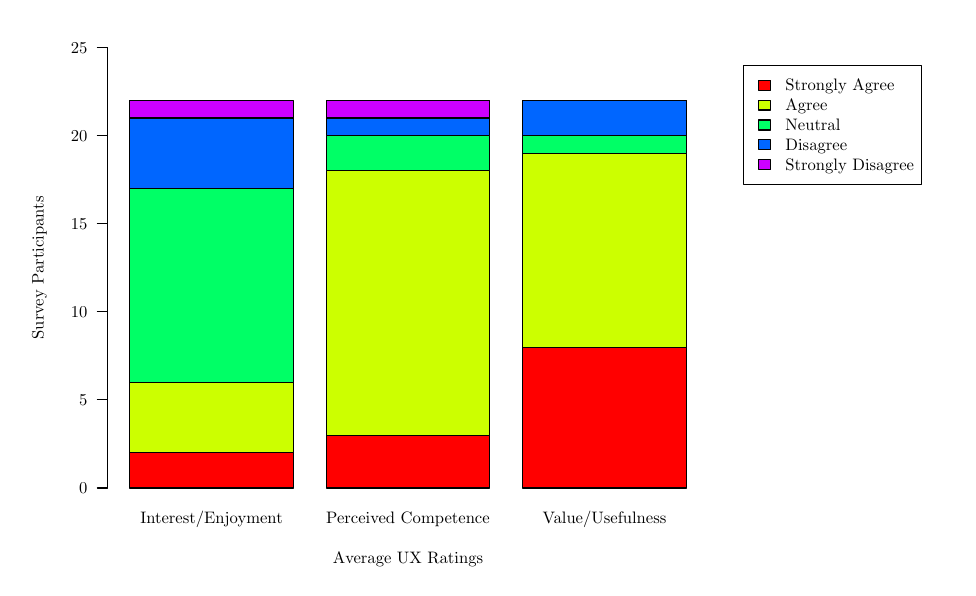
\begin{tikzpicture}[x=1pt,y=1pt]
\definecolor[named]{fillColor}{rgb}{1.00,1.00,1.00}
\path[use as bounding box,fill=fillColor,fill opacity=0.00] (0,0) rectangle (332.44,195.13);
\begin{scope}
\path[clip] (  0.00,  0.00) rectangle (332.44,195.13);
\definecolor[named]{drawColor}{rgb}{0.00,0.00,0.00}
\definecolor[named]{fillColor}{rgb}{1.00,0.00,0.00}

\path[draw=drawColor,line width= 0.4pt,line join=round,line cap=round,fill=fillColor] ( 36.85, 28.80) rectangle ( 96.01, 41.53);
\definecolor[named]{fillColor}{rgb}{0.80,1.00,0.00}

\path[draw=drawColor,line width= 0.4pt,line join=round,line cap=round,fill=fillColor] ( 36.85, 41.53) rectangle ( 96.01, 66.99);
\definecolor[named]{fillColor}{rgb}{0.00,1.00,0.40}

\path[draw=drawColor,line width= 0.4pt,line join=round,line cap=round,fill=fillColor] ( 36.85, 66.99) rectangle ( 96.01,137.01);
\definecolor[named]{fillColor}{rgb}{0.00,0.40,1.00}

\path[draw=drawColor,line width= 0.4pt,line join=round,line cap=round,fill=fillColor] ( 36.85,137.01) rectangle ( 96.01,162.47);
\definecolor[named]{fillColor}{rgb}{0.80,0.00,1.00}

\path[draw=drawColor,line width= 0.4pt,line join=round,line cap=round,fill=fillColor] ( 36.85,162.47) rectangle ( 96.01,168.83);
\definecolor[named]{fillColor}{rgb}{1.00,0.00,0.00}

\path[draw=drawColor,line width= 0.4pt,line join=round,line cap=round,fill=fillColor] (107.84, 28.80) rectangle (167.00, 47.90);
\definecolor[named]{fillColor}{rgb}{0.80,1.00,0.00}

\path[draw=drawColor,line width= 0.4pt,line join=round,line cap=round,fill=fillColor] (107.84, 47.90) rectangle (167.00,143.37);
\definecolor[named]{fillColor}{rgb}{0.00,1.00,0.40}

\path[draw=drawColor,line width= 0.4pt,line join=round,line cap=round,fill=fillColor] (107.84,143.37) rectangle (167.00,156.10);
\definecolor[named]{fillColor}{rgb}{0.00,0.40,1.00}

\path[draw=drawColor,line width= 0.4pt,line join=round,line cap=round,fill=fillColor] (107.84,156.10) rectangle (167.00,162.47);
\definecolor[named]{fillColor}{rgb}{0.80,0.00,1.00}

\path[draw=drawColor,line width= 0.4pt,line join=round,line cap=round,fill=fillColor] (107.84,162.47) rectangle (167.00,168.83);
\definecolor[named]{fillColor}{rgb}{1.00,0.00,0.00}

\path[draw=drawColor,line width= 0.4pt,line join=round,line cap=round,fill=fillColor] (178.83, 28.80) rectangle (238.00, 79.72);
\definecolor[named]{fillColor}{rgb}{0.80,1.00,0.00}

\path[draw=drawColor,line width= 0.4pt,line join=round,line cap=round,fill=fillColor] (178.83, 79.72) rectangle (238.00,149.74);
\definecolor[named]{fillColor}{rgb}{0.00,1.00,0.40}

\path[draw=drawColor,line width= 0.4pt,line join=round,line cap=round,fill=fillColor] (178.83,149.74) rectangle (238.00,156.10);
\definecolor[named]{fillColor}{rgb}{0.00,0.40,1.00}

\path[draw=drawColor,line width= 0.4pt,line join=round,line cap=round,fill=fillColor] (178.83,156.10) rectangle (238.00,168.83);
\definecolor[named]{fillColor}{rgb}{0.80,0.00,1.00}

\path[draw=drawColor,line width= 0.4pt,line join=round,line cap=round,fill=fillColor] (178.83,168.83) rectangle (238.00,168.83);
\end{scope}
\begin{scope}
\path[clip] (  0.00,  0.00) rectangle (332.44,195.13);
\definecolor[named]{drawColor}{rgb}{0.00,0.00,0.00}

\node[text=drawColor,anchor=base,inner sep=0pt, outer sep=0pt, scale=  0.60] at ( 66.43, 15.84) {Interest/Enjoyment};

\node[text=drawColor,anchor=base,inner sep=0pt, outer sep=0pt, scale=  0.60] at (137.42, 15.84) {Perceived Competence};

\node[text=drawColor,anchor=base,inner sep=0pt, outer sep=0pt, scale=  0.60] at (208.42, 15.84) {Value/Usefulness};
\end{scope}
\begin{scope}
\path[clip] (  0.00,  0.00) rectangle (332.44,195.13);
\definecolor[named]{drawColor}{rgb}{0.00,0.00,0.00}

\node[text=drawColor,anchor=base,inner sep=0pt, outer sep=0pt, scale=  0.60] at (137.42,  1.44) {Average UX Ratings};

\node[text=drawColor,rotate= 90.00,anchor=base,inner sep=0pt, outer sep=0pt, scale=  0.60] at (  5.76,108.36) {Survey Participants};
\end{scope}
\begin{scope}
\path[clip] (  0.00,  0.00) rectangle (332.44,195.13);
\definecolor[named]{drawColor}{rgb}{0.00,0.00,0.00}

\path[draw=drawColor,line width= 0.4pt,line join=round,line cap=round] ( 28.80, 28.80) -- ( 28.80,187.93);

\path[draw=drawColor,line width= 0.4pt,line join=round,line cap=round] ( 28.80, 28.80) -- ( 25.20, 28.80);

\path[draw=drawColor,line width= 0.4pt,line join=round,line cap=round] ( 28.80, 60.63) -- ( 25.20, 60.63);

\path[draw=drawColor,line width= 0.4pt,line join=round,line cap=round] ( 28.80, 92.45) -- ( 25.20, 92.45);

\path[draw=drawColor,line width= 0.4pt,line join=round,line cap=round] ( 28.80,124.28) -- ( 25.20,124.28);

\path[draw=drawColor,line width= 0.4pt,line join=round,line cap=round] ( 28.80,156.10) -- ( 25.20,156.10);

\path[draw=drawColor,line width= 0.4pt,line join=round,line cap=round] ( 28.80,187.93) -- ( 25.20,187.93);

\node[text=drawColor,anchor=base east,inner sep=0pt, outer sep=0pt, scale=  0.60] at ( 21.60, 26.73) {0};

\node[text=drawColor,anchor=base east,inner sep=0pt, outer sep=0pt, scale=  0.60] at ( 21.60, 58.56) {5};

\node[text=drawColor,anchor=base east,inner sep=0pt, outer sep=0pt, scale=  0.60] at ( 21.60, 90.39) {10};

\node[text=drawColor,anchor=base east,inner sep=0pt, outer sep=0pt, scale=  0.60] at ( 21.60,122.21) {15};

\node[text=drawColor,anchor=base east,inner sep=0pt, outer sep=0pt, scale=  0.60] at ( 21.60,154.04) {20};

\node[text=drawColor,anchor=base east,inner sep=0pt, outer sep=0pt, scale=  0.60] at ( 21.60,185.86) {25};
\end{scope}
\begin{scope}
\path[clip] (  0.00,  0.00) rectangle (332.44,195.13);
\definecolor[named]{drawColor}{rgb}{0.00,0.00,0.00}

\path[draw=drawColor,line width= 0.4pt,line join=round,line cap=round] (258.70,181.56) rectangle (323.00,138.36);
\definecolor[named]{fillColor}{rgb}{1.00,0.00,0.00}

\path[draw=drawColor,line width= 0.4pt,line join=round,line cap=round,fill=fillColor] (264.10,176.16) rectangle (268.42,172.56);
\definecolor[named]{fillColor}{rgb}{0.80,1.00,0.00}

\path[draw=drawColor,line width= 0.4pt,line join=round,line cap=round,fill=fillColor] (264.10,168.96) rectangle (268.42,165.36);
\definecolor[named]{fillColor}{rgb}{0.00,1.00,0.40}

\path[draw=drawColor,line width= 0.4pt,line join=round,line cap=round,fill=fillColor] (264.10,161.76) rectangle (268.42,158.16);
\definecolor[named]{fillColor}{rgb}{0.00,0.40,1.00}

\path[draw=drawColor,line width= 0.4pt,line join=round,line cap=round,fill=fillColor] (264.10,154.56) rectangle (268.42,150.96);
\definecolor[named]{fillColor}{rgb}{0.80,0.00,1.00}

\path[draw=drawColor,line width= 0.4pt,line join=round,line cap=round,fill=fillColor] (264.10,147.36) rectangle (268.42,143.76);

\node[text=drawColor,anchor=base west,inner sep=0pt, outer sep=0pt, scale=  0.60] at (273.82,172.30) {Strongly Agree};

\node[text=drawColor,anchor=base west,inner sep=0pt, outer sep=0pt, scale=  0.60] at (273.82,165.10) {Agree};

\node[text=drawColor,anchor=base west,inner sep=0pt, outer sep=0pt, scale=  0.60] at (273.82,157.90) {Neutral};

\node[text=drawColor,anchor=base west,inner sep=0pt, outer sep=0pt, scale=  0.60] at (273.82,150.70) {Disagree};

\node[text=drawColor,anchor=base west,inner sep=0pt, outer sep=0pt, scale=  0.60] at (273.82,143.50) {Strongly Disagree};
\end{scope}
\end{tikzpicture}
